\documentclass[11pt,a4paper]{article}
\usepackage[margin=0.78in]{geometry}
\usepackage[T1]{fontenc}
\usepackage{lmodern}
\usepackage{microtype}
\usepackage{booktabs}
\usepackage{tabularx}
\usepackage{threeparttable}
\usepackage{graphicx}
\usepackage{xcolor}
\usepackage{amsmath,amssymb}
\usepackage{siunitx}
\usepackage{pgfplots}
\usepackage{caption}
\usepackage{subcaption}
\usepackage{enumitem}
\usepackage{hyperref}
\usepackage[round,authoryear]{natbib}
\usepackage{titlesec}
\usepackage{fancyhdr}
\pgfplotsset{compat=1.18}
\definecolor{navy}{HTML}{19324D}
\definecolor{orange}{HTML}{B45309}
\definecolor{teal}{HTML}{147D75}
\hypersetup{colorlinks=true,linkcolor=navy,citecolor=navy,urlcolor=navy,pdfauthor={},pdftitle={Dynamic Characteristic Clouds and Cross-Sectional Return Prediction},pdfsubject={}}
\titleformat{\section}{\large\bfseries\color{navy}}{\thesection}{0.6em}{}
\titleformat{\subsection}{\normalsize\bfseries}{\thesubsection}{0.6em}{}
\setlist{nosep,leftmargin=1.3em}
\captionsetup{font=small,labelfont=bf}
\sisetup{detect-all,round-mode=places,round-precision=3}
\pagestyle{fancy}
\fancyhf{}
\fancyhead[L]{Cross-Sectional Return Prediction}
\fancyhead[R]{\thepage}
\renewcommand{\headrulewidth}{0.3pt}
\setlength{\parindent}{0pt}
\setlength{\parskip}{0.45em}

\begin{document}
\begin{titlepage}
\centering
\vspace*{2.5cm}
{\Huge\bfseries Dynamic Characteristic Clouds and Cross-Sectional Return Prediction\par}
\vspace{0.8cm}
{\Large Big Data Analytics Research Project\par}
\vspace{1.5cm}
{\large Sandhya Jaikumar\par}
\vfill
{\large Sample: United States equities, 1980--2024\par}
{\large Out-of-sample evaluation: 1999--2024\par}
\vspace{1.5cm}
\end{titlepage}

\section*{Executive Summary}

\subsection*{Research objective and investment hypothesis}

This project asks whether representing the monthly equity market as a dynamic cloud of firms in characteristic space improves cross-sectional return prediction and long--short portfolio performance. Monthly US stock observations from 1980--2024 are used to predict next-month excess returns. The investable research universe requires a valid CRSP PERMNO and a micro, small, large or mega size classification; nano stocks are excluded. Characteristics are ranked within each signal month and mapped to $[-1,1]$ before target availability is inspected. This preserves the contemporaneous cross-section and prevents missing future returns from influencing preprocessing.

The investment hypothesis is that expected returns may depend on a firm's relative position in the market-wide characteristic distribution and how that position changes. The analysis tests whether jointly modelling firms improves on independent-stock prediction, whether lagged locations and velocities improve static set models, whether gains appear in both forecasts and portfolios, and whether characteristic breadth has diminishing marginal value.

\subsection*{Data, characteristics and out-of-sample design}

Core20 was selected for broad economic coverage rather than concentration in one anomaly family. It spans size and value, momentum and reversal, profitability and quality, investment and financing, risk, liquidity and trading activity. Four additional mixed blocks of 20 characteristics were fixed before the breadth experiment.

All results are genuinely out of sample. Each annual refit uses 15 years for training, four for validation and the following year for testing. This produces 26 test years (1999--2024), 312 monthly portfolios and 1,323,218 stock forecasts per model. Hyperparameters and early stopping use validation data only. The primary statistical metric is the Gu, Kelly and Xiu zero-benchmark out-of-sample statistic
\[
R^2_{\mathrm{OOS}}=1-\frac{\sum_{i,t}(r_{i,t+1}-\widehat r_{i,t+1})^2}{\sum_{i,t}r_{i,t+1}^2}.
\]
Economic value is measured using a prespecified equal-weight portfolio that buys the top predicted decile and shorts the bottom predicted decile each month.

\subsection*{Model development}

The model set includes LASSO, LightGBM, XGBoost and feedforward neural-network benchmarks; static, lagged and dynamic DeepSets; lagged-characteristic tree models; and validation-only hybrid models. Tree models initially use current monthly characteristic ranks. Temporal versions add the firm's ranks from the immediately preceding month; velocity is current rank minus lagged rank.

Set-based models process the whole month as an unordered collection of firms. DeepSets applies a shared encoder to every stock and combines each stock representation with a leave-one-out market embedding. The dynamic cloud treats each firm as a moving point in the monthly characteristic distribution, using current locations, lagged locations and velocities. Hybrid models test whether DeepSets information is more useful as relative coordinates or as a validation-weighted component of LightGBM.

\subsection*{Headline results and model selection}

\begin{table}[ht]
\centering\small
\caption{Principal out-of-sample results}
\label{tab:main}
\begin{tabular}{lrrrrr}
\toprule
Model & OOS $R^2$ (\%) & Rank IC & Return (\%) & Sharpe & NW $t$ \\
\midrule
LGBM\_40 & 0.294 & 0.052 & 28.51 & \textbf{1.67} & 5.68 \\
LGBM\_CORE & 0.315 & 0.062 & 28.25 & 1.42 & 5.46 \\
XGBOOST\_CORE & 0.233 & 0.060 & 26.62 & 1.35 & 5.21 \\
DEEPSET\_CORE & 0.257 & 0.062 & 26.95 & 1.35 & 4.56 \\
DEEPSET\_LAG\_CLOUD & -0.138 & 0.062 & 26.42 & 1.42 & 5.32 \\
DEEPSET\_DYNAMIC\_CLOUD & -0.241 & 0.052 & 26.01 & 1.50 & 5.07 \\
NN3\_CORE & 0.121 & 0.054 & 19.14 & 0.99 & 3.75 \\
LASSO\_CORE & 0.176 & 0.072 & 17.38 & 0.72 & 3.00 \\
\bottomrule
\end{tabular}
\end{table}

LGBM\_40 is selected as the main model because it provides the best observed Sharpe ratio (1.67) while retaining positive OOS $R^2$, robust OOS $R^2$, significant rank IC and comparatively low drawdown. Its annualized long--short return is 28.5\%, volatility is 17.1\%, the Newey--West $t$-statistic is 5.68 and maximum drawdown is $-28.1$\%. Pairwise inference is more cautious than the raw ranking: none of the six planned long--short return differences is significant after multiple-testing adjustment, and no Sharpe-difference bootstrap interval excludes zero. LGBM\_40 is therefore the most balanced model, not a statistically proven universal winner.

Selection considered forecasting accuracy, ranking quality, economic performance, stability and complexity jointly. LGBM\_40 also has complete signal availability and strongly ordered decile returns: the Spearman correlation across the ten mean decile returns is 0.976 and 77.8\% of adjacent movements are increasing. Its spread is not solely produced by anomalous endpoint portfolios.

\subsection*{Characteristic breadth}

\begin{figure}[ht]
\centering
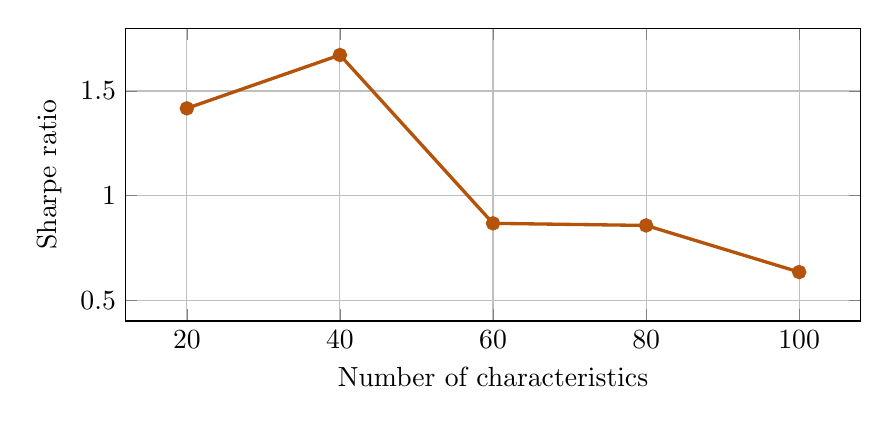
\begin{tikzpicture}
\begin{axis}[width=.9\linewidth,height=5.3cm,xlabel={Number of characteristics},ylabel={Sharpe ratio},xtick={20,40,60,80,100},grid=major,ymin=0.4,ymax=1.8]
\addplot[color=orange,very thick,mark=*] coordinates {(20,1.417) (40,1.672) (60,0.867) (80,0.857) (100,0.634)};
\end{axis}
\end{tikzpicture}
\caption{Feature breadth has an inverted-U relationship with economic performance.}
\label{fig:breadth}
\end{figure}

The mandatory characteristic expansion produces a clear inverted-U pattern. Moving from 20 to 40 mixed characteristics raises Sharpe from 1.42 to 1.67 even though OOS $R^2$ and rank IC fall slightly. Expanding to 60, 80 and 100 characteristics produces negative OOS $R^2$, Sharpe below 0.87 and 14 no-signal months in each specification. More data are therefore valuable only when the marginal characteristics add stable information rather than estimation noise.

\subsection*{Does the dynamic characteristic cloud help?}

The cloud evidence is nuanced. Relative to static DeepSets, lagged and dynamic cloud models improve observed Sharpe, with the dynamic model reaching 1.50 and lowering volatility to 17.3\%. However, both have negative OOS $R^2$. After Holm adjustment, static DeepSets has significantly better MSE and rank IC than dynamic DeepSets, while lag-cloud DeepSets also has significantly better rank IC than the dynamic version. The cloud representation improves economic portfolio separation in the observed sample but does not improve calibrated return forecasts or whole-universe ordering. The main research hypothesis is therefore only partially supported.

The direct answer is qualified: dynamic representation improves observed portfolio risk and Sharpe within the DeepSets family, but worsens OOS $R^2$ and whole-universe ranking and does not surpass the best LightGBM benchmark.

\subsection*{Regime stability and economic mechanism}

\begin{table}[ht]
\centering\small
\caption{LGBM\_40 stability across signal-date volatility regimes}
\label{tab:regime}
\begin{tabular}{lrrrrrr}
\toprule
Regime & Months & Return (\%) & Vol. (\%) & Sharpe & NW $t$ & Rank IC \\
\midrule
High volatility & 174 & 34.02 & 20.62 & 1.65 & 4.11 & 0.058 \\
Low volatility & 138 & 21.57 & 10.78 & 2.00 & 6.82 & 0.045 \\
\bottomrule
\end{tabular}
\end{table}

The selected model is stable across market environments. Returns and rank IC remain positive in both high- and low-volatility regimes. High-volatility months generate stronger raw return separation, while low-volatility months deliver the higher Sharpe, hit rate and lower drawdown. Feature logic is also stable. The model rewards medium-term momentum, R\&D intensity, cash-flow value and profitability in both regimes, while penalizing very recent returns, lottery-like maximum returns and rapid asset growth. Nine of the ten most influential characteristics appear in both regimes.

\subsection*{Factor attribution and implementability}

Factor attribution indicates that the strategy is not simply market exposure. An FF5-plus-momentum regression estimates monthly alpha of 1.97\% (23.6\% annualized) with a HAC $t$-statistic of 7.58. The portfolio has significant profitability, value and momentum loadings, so the residual should not be described as ``pure'' alpha; nevertheless, standard factors do not explain most of the average spread. The long leg contributes 18.1 percentage points and the short leg 10.4 points to the 28.5\% annualized return.

\begin{table}[ht]
\centering\small
\caption{Implementability robustness at 25 basis points per unit of turnover}
\label{tab:costs}
\begin{tabular}{llrr}
\toprule
Universe & Weighting & Net return (\%) & Net Sharpe \\
\midrule
Full & Equal & 25.67 & 1.51 \\
Full & Value & 13.75 & 0.58 \\
Ex-microcap & Equal & 11.11 & 0.51 \\
Ex-microcap & Value & 9.77 & 0.43 \\
\bottomrule
\end{tabular}
\end{table}

The principal limitation is implementability. Returns remain positive after proportional costs, excluding microcaps and applying value weights, but the decline is economically large. The headline result depends materially on smaller stocks, where spreads, market impact and short-borrow constraints are greatest. The full equal-weight portfolio should therefore be interpreted as evidence of predictable cross-sectional return separation rather than directly achievable institutional performance.

\subsection*{Recommendation and limitations}

A client should treat LGBM\_40 as the preferred research strategy, subject to explicit liquidity controls. Implementation should focus initially on the more liquid universe, use conservative trading and borrowing assumptions, and monitor rank IC, feature contributions, turnover and no-signal months. Dynamic cloud models should remain research extensions rather than replacing the selected benchmark.

The conclusions are limited by microcap dependence, equal-weight sensitivity, simplified proportional costs, unavailable security-level borrow and market-impact data, specification-search risk and the fact that historical significance does not guarantee future alpha.

Overall, the evidence favours a parsimonious nonlinear model with a moderately expanded characteristic set. Dynamic cloud information is economically interesting and improves the DeepSets risk profile, but it does not dominate conventional benchmarks. The strongest client proposition is LGBM\_40: a stable, interpretable and statistically credible forecasting model whose economic value survives conservative robustness tests, subject to meaningful liquidity and capacity limitations.

\clearpage
\appendix
\section{Technical Appendix}

\subsection{Data construction, cleaning and universe}
The target is next-month excess return, \texttt{ret\_exc\_lead1m}. Signal-month characteristics are ranked across all eligible firms before rows with unavailable future returns are identified. Missing ranks are filled with zero. The universe includes US observations with valid PERMNO and size group micro, small, large or mega; nano observations are excluded. Both \texttt{id} and PERMNO are retained, and uniqueness of $(\text{eom},\text{PERMNO})$ is enforced. The saved target date is exactly one month-end after the signal date.

\subsection{Rolling schedule and information timing}
The rolling design uses 15 calendar years of training, four validation years and one test year. Test year 1999 uses 1980--1994 for training and 1995--1998 for validation. The window moves forward by one year and the model is refitted annually through 2024. Validation MSE determines regularization, early stopping and tree iteration. Test outcomes never influence model or hyperparameter selection.

\subsection{Core benchmark and set-model specifications}
LASSO is a sparse linear baseline. LightGBM and XGBoost use squared-error regression on independent stock-month rows. NN3 is a three-hidden-layer feedforward benchmark. MLP\_40 is the matched no-market-context neural control. DeepSets treats each month as an unordered set of firms: a shared stock encoder is combined with a leave-one-out monthly market embedding.

\subsection{Temporal, cloud and hybrid specifications}
DEEPSET\_LAG\_CLOUD augments current Core20 ranks with exact-calendar one-month lags and an availability flag. DEEPSET\_DYNAMIC\_CLOUD additionally includes velocity, defined as current rank minus lagged rank. Lags are constructed on the complete eligible panel before target filtering. A firm returning after a gap receives neutral lag values and an unavailable flag.

LGBM\_20/40/60/80/100 form the required breadth experiment using frozen mixed blocks. LGBM\_40\_LAG1 adds exact one-month lags for the selected 40-characteristic set. Hybrid and recalibrated models use validation-only combination rules and are interpreted as robustness experiments when introduced after initial results.

\subsection{Statistical forecasting diagnostics}
Monthly rank IC is the cross-sectional Spearman correlation between forecast and realized next-month return, requiring at least 20 finite outcomes. Constant forecasts produce undefined IC and no-signal portfolio months hold cash; PERMNO is never used to manufacture a ranking. Inference includes conventional, Newey--West and test-year-clustered statistics, as appropriate. Robust OOS $R^2$ clips predictions and outcomes within month at the 0.5\% and 99.5\% quantiles; the unmodified GKX statistic remains primary.

\subsection{Portfolio formation and implementation tests}
The headline portfolio sorts all eligible predictions before target availability is inspected, then calculates equal-weight realized D10 minus D1. Alternative 5\%, 20\% and rank-weighted portfolios are sensitivities. Transaction-cost robustness applies costs to intended signed-weight turnover and evaluates full/ex-microcap and equal/value-weighted portfolios. It excludes security-specific spreads, nonlinear impact and borrow fees.

\subsection{Paired inference}
Six planned comparisons use monthly paired observations. MSE and portfolio-return differences use Newey--West inference; rank-IC differences use test-year clustering; Sharpe differences use test-year block-bootstrap intervals. Holm adjustment is applied within each family. Differences are model A minus model B, so a negative MSE difference favours model A.

\begin{table}[ht]
\centering\scriptsize
\caption{Holm-adjusted paired findings}
\begin{tabularx}{\linewidth}{XXrrr}
\toprule
Model A & Model B & MSE $p$ & Return $p$ & Rank-IC $p$ \\
\midrule
LGBM\_40 & LGBM\_CORE & 1.000 & 1.000 & 0.041 \\
LGBM\_40 & LGBM\_40\_LAG1 & 1.000 & 1.000 & 0.201 \\
LGBM\_40 & DEEPSET\_DYNAMIC\_CLOUD & 0.163 & 1.000 & 1.000 \\
DEEPSET\_CORE & DEEPSET\_LAG\_CLOUD & 0.826 & 1.000 & 1.000 \\
DEEPSET\_CORE & DEEPSET\_DYNAMIC\_CLOUD & 0.016 & 1.000 & 0.014 \\
DEEPSET\_LAG\_CLOUD & DEEPSET\_DYNAMIC\_CLOUD & 1.000 & 1.000 & 0.038 \\
\bottomrule
\end{tabularx}
\end{table}

\subsection{Regime and feature analysis}
The market regime is based on trailing 12-month volatility of a beginning-market-equity-weighted market excess return. Current trailing volatility is compared with an expanding historical median shifted by one month. This classification uses signal-date information only. Exact annual LightGBM checkpoints generate out-of-sample contribution values. Absolute contribution identifies importance; signed contribution, within-month rank association and the top-minus-bottom feature-quintile contribution describe direction. No replacement model is fitted.

\subsection{Factor decomposition}
The 10\% long--short return is aligned to its realization month and regressed on the Fama--French five factors plus momentum. Newey--West standard errors use six lags. Estimated loadings are: market $-0.092$, size $0.136$, value $0.279$, profitability $0.906$, investment $0.190$ and momentum $0.161$. Value, profitability and momentum are statistically significant at conventional levels.

\subsection{Artifact integrity and reproducibility}
The final audit verifies all 20 models, 26 annual refits, 312 OOS months, prediction schema, unique keys, signatures, target timing and exact portfolio reconstruction. The frozen chosen-model signature is \texttt{c7e5a69df65fab9c}. Every model contains 1,323,218 predictions and uses diagnostic version \texttt{post\_model\_v4\_signal\_cash}.

\subsection{Limitations}
The study is subject to model-search risk because multiple architectures and feature variants were investigated. Pairwise inference and the distinction between original tournament models and post-hoc robustness models mitigate but do not eliminate this issue. Delisting treatment and return-field construction inherit the source dataset conventions. The cost exercise is not a capacity model, and the strong dependence on microcaps restricts institutional interpretation. Finally, factor-adjusted alpha is an ex-post attribution, not a guarantee of future abnormal performance.

\bibliographystyle{plainnat}
\bibliography{references}
\end{document}
